\chapter{Комплексная оценка производительности ВС}

В настоящий момент списки Top50 и Top500
выстроены в порядке убывания пиковой производительности и производительности на тесте LinPack что, разумеется, дает определенную информацию
о сравнительной скорости работы представленных там машин. Но очень многие факторы, такие как скорость работы и объем дисков, пропускная 
способность шины памяти и коммуникационной сети, неоднородность оборудования и т.д. - остаются за пределами рассмотрения. А это именно те 
проблемы, с которыми придется столкнуться при попытке посчитать на кластере большую задачу. По этой причине тестирование продится с помощью измерения времени, затрачитваемого на различные этапы программы, решающей реальную физическую задачу.

В \textbf{третьей главе} описана методика измерения характеристик ВС с помощью программы, реализующей метод частиц в ячейках.


\textbf{везде написать пиковые знач. - Курносов 
}


Предложена методика комплексной оценки тестируемой ВС с точки зрения возможности эффективной реализзации математических моделей на основе определения баланса между скоростью счета и скоростью пересылки данных между узлами ВС. Баланс определяется на основе усреднения данных расчетов по методу частиц в ячейках, который используется в качестве оценки снизу по скорости счета и оценки сверху по памяти для большинства существующих математических методов.

Кроме того, на основе проведенных расчетов измерена скорость счета и скорость перемещения данных для нескольких протестированных ВС.   

		
\textbf{сделать общий список всех расчетов, упоминающихся в..., для каждого укказать флопсы, в сравнениии с пиком, место в топ50 (с обясненнеим, почему наше лучше), для кого можно, производительность сети и общую оценку}

\textbf{Таблицу прогнозовов составляйт не только для гибридных, но и для всех, кого можно}





\section{О влиянии организации данных на результат измерения производительности процессоров}
\label{procs_influence}

Модельные частицы расположены внутри расчетной области случайным образом. Если даже модельные частицы расположены рядом в массиве, где хранятся их координаты,  то сами значения координат будут близкими только вначале. В дальнейшем модельные частицы перемешиваются. Это означает, что обращения к трехмерным массивам, содержащим электрическое и магнитное поля, являются неупорядоченными,  и использование кэш-памяти в данном случае не позволяет сократить время счета. 

Использование кэш-памяти было бы более эффективным, если бы частицы были упорядочены. Тогда значения полей, загруженных в кэш при расчете движения некоторой частицы, могли бы быть использованы и для следующей частицы, если она расположена близко. 

Для этого достаточно упорядочить частицы по ячейкам сетки, то есть, хранить каким-то образом вместе все частицы, которые расположены внутри каждой ячейки. Это означает, что полная сортировка массива частиц не нужна, так как с точки зрения использования кэш-памяти не имеет значения, как частицы расположены внутри ячейки. 

Модельные частицы, принадлежащие некоторой ячейке сетки, можно хранить в виде связанного списка или в виде массива. Преимущества списка очевидны: нет ограничения на число частиц в ячейке, простота добавления/удаления, но есть и недостатки, а именно большее по сравнению с массивом время доступа. Если же частицы каждой ячейки хранятся в виде массива (статического массива), то применительно к трехмерной задаче для двух сортов частиц это даст 5-мерный массив для одной только координаты X всех частиц (напомним, что модельная частица в данном случае характеризуется шестью признаками). 

Но основная проблема в случае статического массива - это максимальное число частиц в ячейке. Это означает, что заранее неизвестно, какой длины массив потребуется для хранения всех частиц в каждой ячейке. Из проведенных расчетов известно, что максимальное значение плотности электронов было равно 5 (в единицах начальной плотности). Таким образом, можно было бы задать длину массива частиц в каждой ячейке 5N, где N - число частиц в ячейке в начальный момент времени. Но в этом случае размер массива частиц увеличится в 5 раз, а его размер составляет 70 Гб, например, для сетки 512х64х64 и N = 150. 

Использование для этой цели динамических массивов решает проблему перерасхода памяти, но создает другую: необходимость иметь внутри программы свой эффективный менеджер динамической памяти, что, возможно, является решаемой задачей, но едва ли приведет к существенному уменьшению времени работы программы в целом. 

Поэтому был реализован компромиссный вариант: для каждого сорта частиц (в данном случае 2 сорта: электроны и ионы) в каждой ячейке в целочисленном массиве длины 5N хранить номера частиц, находящихся в данный момент в данной ячейке. Номер задает позицию частицы в больших (порядка 100 млн. элементов) вещественных массивах, в которых хранятся координаты и импульсы модельных частиц. Таким образом, при перемещении частицы из одной ячейки в другую (обязательно в соседнюю - это определяется соображениями устойчивости метода частиц) перемещается только номер частицы: он удаляется из массива номеров, описывающих текущую ячейку, и добавляется в массив номеров одной из соседних ячеек. Внутри самих массивов координат и импульсов частицы никогда не перемещаются. 

Также был реализован вариант с хранением частиц каждой ячейки в виде связанного списка. В этом случае имеется 4-мерный массив указателей, задающий первый элемент списка в каждой ячейке, и отсутствуют большие массивы: вся информация по частицам хранится только в списках. 

В обоих вариантах на вход процедуры интегрирования уравнений движения модельных частиц подаются шесть небольших (размером не более 5N) массивов, хранящих координаты и импульсф частиц для каждой конкретной ячейки. Эти массивы формируются либо на основе списка частиц, либо на основе массива номеров частиц этой ячейки. 

Таким образом, имеются следующие варианты организации частиц в программе:
\begin{enumerate}
	\item Исходный неоптимизированный вариант; 
	\item Хранение значений поля в 4-мерном массиве; 
	\item Упорядочивание частиц с помощью массивов номеров; 
	\item Упорядочивание частиц с помощью связанного списка; 
\end{enumerate}

Далее рассмотрим результаты тестов, показывающих эффективность выполненной оптимизации. Тестовые расчеты проводились на рабочей станции с процессором AMD Phenom (Phenom II X6 1055T),  производительность\footnote{https://www.techpowerup.com/forums/threads/processor-gflops-compilation.94721/} 41.9 GFLOPS), и на кластере Новосибирского Государственного Университета, оснащенного процессорами процессор Intel Xeon  E5540 (производительность\footnote{http://browser.geekbench.com/geekbench2/413456} на LU-разложении 2.5 GFLOPS). В обоих случая была выбрана сетка такого размера, что даже один трехмерный массив, содержащий, например, одну из компонент поля, заведомо не помещается в кэш. 
Размер сетки для рабочей станции на базе процессора Phenom  $64\times32\times32$ узла, 150 частиц в ячейке, всего 9.8 млн. частиц. Размер сетки для кластера на базе процессора Intel Xeon  E5540 в расчете на одно ядро, $512\times2\times64$ узла, 150 частиц в ячейке, те же 9.8 млн. частиц на ядро. С учетом определенного в главе 1 количества операций в расчете на одну частицу (около 500) можно рассчитать производительность в единицах GFLOPS.

\begin{table}[ht]
	\label{part_optim}
	\begin{center}
		\caption{Время вычислений,  в секундах, и производительность, GFLOPS.}
		\begin{tabular}{|c|c|c|c|c|c|}
\hline			

&& \multicolumn{2}{|c|}{Время} &	
   \multicolumn{2}{|c|}{Производительность}		\\		\cline{3-4} \cline{5-6}
№ &		 Вариант оптимизации                      & Phenom & Xeon  E5540  & Phenom & Xeon  E5540\\ \hline   	
1&Исходный                                          &        &            &        &            \\ 
 &неоптимизированный вариант                        & 13.25  & 7.22       &  0.369 & 0.67           \\ \hline  
2&Хранение значений поля                            &        &            &        &            \\
 & в 4-мерном массиве                               & 8.8    & 6.72       &  0.55  & 0.72       \\ \hline
3&Упорядочивание частиц                             &        &            &        &            \\ 
 & с помощью массивов номеров                       & 12.51  & 5.67       &  0.39  & 0.86           \\ \hline
4 &Упорядочивание частиц                             &        &           &        &            \\   
  & с помощью связанного списка                      & 10.5   & 10.3      &  0.46  & 0.475           \\ \hline
5 &                                                  &        &           &        &            \\
  &Сочетание вариантов 2 и 3			              & 10.92  & 3.67     &  0.44  & 1.33       \\ \hline 
		
\end{tabular}
\end{center}
\end{table}			



Отсюда можно сделать вывод, что сочетание упорядочивания модельных частиц и хранения значений поля в одном 4-мерном массиве приводит к значительному сокращению времени вычислений с частицами, в данном случае, почти в 2 раза. Хранение частиц в виде связанных списков оказалось неэффективным для процессора Xeon  E5540, но, возможно, окажется полезным на других архитектурах (так позволяют думать измерения времени на процессоре Phenom)или в тех случаях, когда установить максимальное число частиц в ячейке невозможно.

Относительно небольшая доля от пиковой производительности, полученная в этих тестах, показывает значительную разницу между расчетом по методу частиц в ячейках, и например, методами решения линейных уравнений, которые являются наиболее распространенным тестом производительности ВС. Это подчеркивает необходиость отдельного тестирования также и на методе частиц в ячейках, и кроме того, подчеркивает важность также и проверки в рамках тестов не только производительности, но и скорости доступа к оперативной памяти, что будет предметом рассмотрения в одном из следующих разделов (раздел \ref{perfRAM}). 

Основная ценность этих экспериментов в том, что установлено влияние, которое способ организации частиц в памяти оказывает на производительность, а значит и на результаты работы создаеваемой программы-теста, например, какое влияние на результат тестирования может оказать более или менее эффективно работающий кэш: по результатам, показанным в таблице \ref{part_optim}, производительность может измениться н более чем в 1.5-2 раза.


\section{Расчет производительности системы памяти}
\label{perfRAM}
Вэтом разделе описано измерение производительности системы памяти, основанное на измерении времени расчета движения модельных частиц, при этом благодаря алгоритмически особенностям метода частиц в ячейках удается исключить использование кэш-памяти и производить измерение скорости доступа именно к оперативной памяти.

\begin{table}[ht]
\caption{
Основные характеристики кластеров, на которых производились расчеты,рассмотренные в разделах \ref{perfRAM},\ref{calc_PE} и \ref{perfCommNet}, Номера даны по списку Top50 от 2009 года, В колонке TFLOPS указана пиковая производительность в терафлопсах.}
	\begin{center}
		\begin{tabular}{|c|c|c|c|c|}
			\hline
			№                 & Название & Узлы               & Сеть                                   &  TFlOPS\\
		          \hline 
			1                & МВС-100К & 4xXeon E5450,      &  Infiniband 4x DDR/                    & 95.04 \\
			&          & 3 GHz              &  2xGigabit Ethernet/                   &       \\
			&          & 8.192 GB RAM       &  Gigabit Ethernet                      &    \\ \hline 
			2                 & СКИФ-МГУ & 2xXeon E5472,      & InfiniBand/                             & 60   \\
			&          &   3 GHz            & Gigabit Ethernet/                       &      \\
			&          &  8.192 GB RAM      & СКИФ-ServNet + IPMI                    &   \\ \hline 
			14                & СКИФ-Cyberia & 2xXeon 5150,   &  QLogic InfiniPath/                     & 12.002 \\
			&              &  2.667 GHz,    & Gigabit Ethernet/                       &   \\
			&           &     4.096 GB RAM  & СКИФ-ServNet                            & \\ \hline 
			20                & Кластер НГУ & 2xXeon 5355,    &  Infiniband 4x DDR/                    & 5.4 \\ 
			&           & 2.66 GHz          &   Gigabit Ethernet/                    &  \\
			&           &                   &   Gigabit Ethernet                     &  \\ \hline 
			
		\end{tabular}
	\end{center}

	\label{top50_2010}
\end{table}

Переход от фактически измеренной величины, времени выполнения расчета движения модельных частиц выполнялся из следующих соображений: на каждое из используемых ядер приходится 2.5 млн. модельных частиц, каждая частица занимает 48 байт, кроме того, для расчета движения частицы необходимы значения электрического и магнитного полей в той ячейке сетки, где находится частица. Это означает, что для каждой из 6 компонент электромагнитного поля загружается 8 значений, соответствующих вершинам параллелепипеда, то есть ячейки сетки. 

Более того, по результатам расчета движения модельной частицы вычисляется вклад данной частицы в ток. Для каждой из трех меняются значения в 4 узлах сетки компоненты тока, которые вместе с новыми значениями координаты и импульса модельной частицы сохраняются в оперативную память.

Таким образом для каждой модельной частицы загружается из памяти 432 байта и сохраняется 144 байта, общий поток данных составляет 576 байт на одну частицу.

В итоге, для вычисления пропускной способности памяти (в GB/sec) при расчете движения модельных частиц $W_{PIC,GB/sec}$ использовалась следующая формула:
\begin{equation}
W_{PIC,GB/sec} = \frac{W_P\times N_P P_{core}}{\Delta t}
\label{RAM_performance}
\end{equation}
здесь:
\begin{itemize}
	\item $W_P$ - количество байт на одну модельную частицу, $W_P = 576$;
	\item $N_P$ - количество модельных частиц на одно процессорное ядро (в рассмотренном случае $2.5\times 10^6$);  
	\item $P_core$ - количество процессорных ядер;
	\item $\Delta t$  - длительность временного шага, сек.
\end{itemize}	




\begin{figure}[htb]
	\begin{center}
		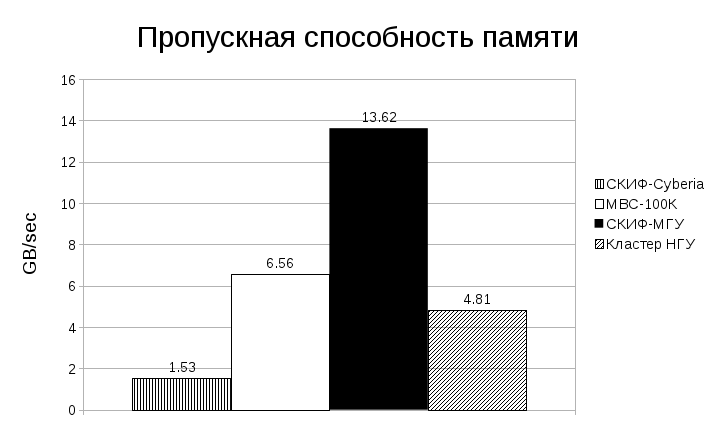
\includegraphics[height=7cm,keepaspectratio]{images/data_proc_throughput_GBsec.png}
	\end{center}
	\caption{Пропускная способность памяти на этапе расчета движения модельных частиц на некоторых кластерах. Количество модельных частиц: 2.5 млн. на каждое процессорное ядро. Основные параметры ВС, использованных в эксперименте, показаны в таблице \ref{top50_2010}.}
	\label{PIC_RAM}
\end{figure}
Следует отметить, что вопрос о сравнении чисел на рис. \ref{PIC_RAM} с заявленной максимальной пропускной способностью 
является второстепенным, тем не менее, сравнение показано в таблице \ref{PIC_vs_PROC_RAM}. Основной вопрос в данном случае - это измерение пропускной способности памяти,  фактически доступной для расчетного приложения.

\begin{table}[ht]
\caption{Сравнение пропускной способности памяти, измеренной с помощью теста на основе метода частиц с характеристиками процессора.}
\label{PIC_vs_PROC_RAM}
\begin{tabular}{|c|c|c|c|}
	\hline
             &            & \multicolumn{2}{|c|}{Пропускная способность памяти, GB/sec} \\ \cline{3-4}  	
Название ВС  & Процессор  & Данные теста MANAS & Максимум \\ \hline
МВС-100К     & Xeon E5450 &     6.02           & 21       \\ \hline 
СКИФ-МГУ     & Xeon E5472 &     12.47          & 21       \\ \hline     
СКИФ-Cyberia & Xeon 5150  &     1.45           & 10.6     \\ \hline
Кластер НГУ  & Xeon 5355  &     4.47           & 21       \\ \hline
\end{tabular}	
\end{table}

\section{Расчет производительности процессорных элементов}
\label{calc_PE}
В \textit{первом разделе} описана методика измерения производительности процессорных элементов.
Для того, чтобы отделить время счета от времени обращения к оперативной памяти было рассмотрено время работы процедуры,
реализующей одномерное преобразование Фурье, которая является частью физической диагностики, используемой в при моделировании динамики плазмы. Измереннное время с учетом известного размера данных и и количества операций в БПФ , переводится во флопсы. Сравнительная производительность процессорных элементов некоторых из рассмотренных в диссертационной работе ВС выглядит как показано на рисунке  \ref{procs_flops}:

\begin{figure}[htb]
	\begin{center}
		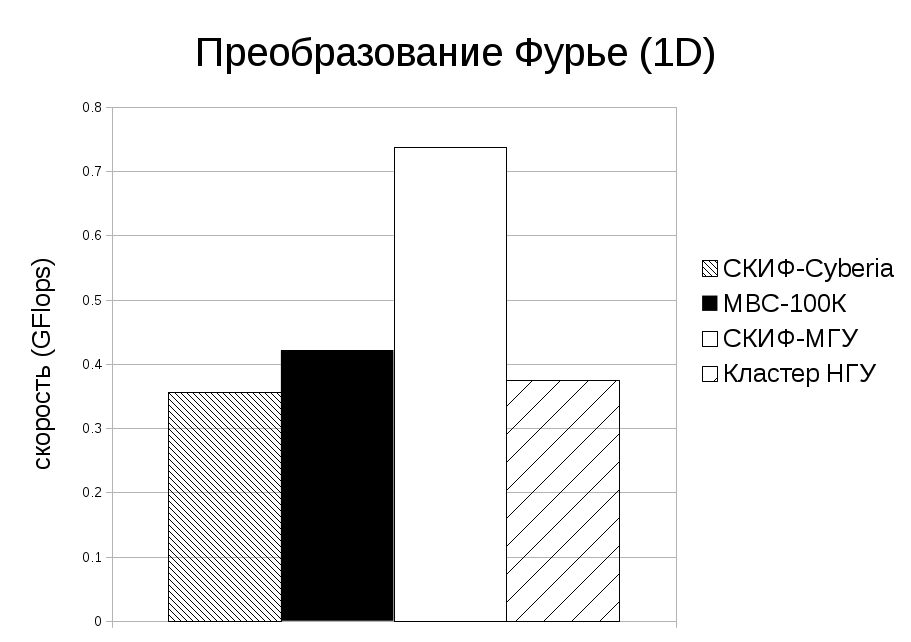
\includegraphics[height=7cm,keepaspectratio]{images/processor_FLOPS.png}
	\end{center}
	\caption{Производительность процессоров Intel Xeon, измеренная в ходе выполнения одномерного преобразования Фурье на некоторых кластерах. Размерность преобразования $N=64$. Измерения выполнены в 2010 г.}
	\label{procs_flops}
\end{figure} 


\section{Расчет производительности процессорных элементов на основе движения модельных частиц}
\label{calc_PE}
 Сравнительная производительность процессорных элементов некоторых из рассмотренных в диссертационной работе ВС выглядит как показано на рисунке  \ref{procs_flops_pic}:

\begin{figure}[htb]
	\begin{center}
		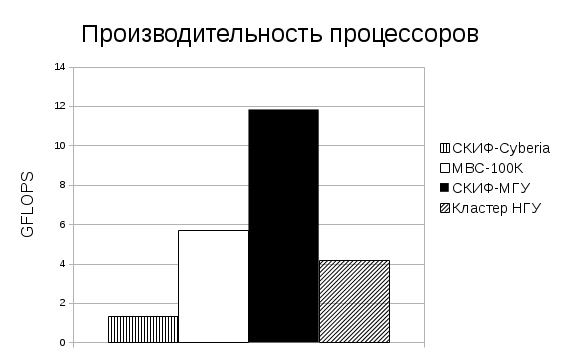
\includegraphics[height=10cm,keepaspectratio]{images/processor_FLOPS_PIC.png}
	\end{center}
	\caption{Производительность процессоров Intel Xeon, измеренная на основе времени вычисления движения модельных частиц. Измерения выполнены в 2010 г.}
	\label{procs_flops_pic}
\end{figure} 

Расчет количества операций с плавающей точкой в секунду (FLOPS) при расчете движения модельных частиц $N_{PIC,FLOPS}$ производился следующим образом:
\begin{equation}
N_{PIC,FLOPS} = \frac{F_P\times N_P \times P_{core}}{\Delta t}
\label{PIC_FLOPS}
\end{equation}

здесь:
\begin{itemize}
	\item $F_P$ - количество операций на одну модельную частицу, $F_P = 500$;
	\item $N_P$ - количество модельных частиц на одно процессорное ядро (в рассмотренном случае $2.5\times 10^6$);  
	\item $P_{core}$ - количество ядер процессора;
	\item $\Delta t$  - длительность временного шага, сек.
\end{itemize}	

\begin{table}[ht]
	\caption{Производительность процессоров Intel Xeon, измеренная на основе времени вычисления движения модельных частиц.}
	\label{PIC_vs_PROC_RAM}
	\begin{tabular}{|c|c|c|c|c|c|}
		\hline
		&            &            &             &       \multicolumn{2}{|c|}{Производительность, GFLOPS} \\ \cline{5-6}  	
		Название ВС  & Процессор  &  $\Delta t$ &$P_{core}$ & Данные теста  &  \\
		             &            &             &           & PIC-MANAS     & LU-разложение \\ \hline
		МВС-100К     & Xeon E5450 &  0.878      & 4     & 5.69           & 4.6     \\ \hline 
		СКИФ-МГУ     & Xeon E5472 &  0.423      & 4     & 11.83          & 2.37       \\ \hline     
		СКИФ-Cyberia & Xeon 5150  &  1.882      & 2     &  1.33          & 4.65    \\ \hline
		Кластер НГУ  & Xeon 5355  &  1.196      & 4     & 4.18           & 1.82       \\ \hline
	\end{tabular}	
\end{table}






\section{Расчет производительности коммуникационной сети}
\label{perfCommNet}
Разработана методика измерения быстродействия коммуникационной сети на основе анализа времени работы MPI-процедур, осуществляющих обмен граничными значениями между отдельными подобластями при решении уравнений Максвелла и при пересылке модельных частиц. В силу того, что при этом используются различные виды коммуникационных функций  - как блокирующие, так и не блокирующие, как парные, так и коллективные, при использовании эйлерово-лагранжевой декомпозиции - это позволяет набрать в течение одного расчета большую базу данных для получения знаний о структуре коммуникационной сети, времени прохождения сообщений в зависимости от размера, системных таймаутах и пр. 

В данном случае показан более простой и более ограниченный тест, полученный на основе измерения времени пересылки модельных частиц, перелетающих из одной подобласти в другую (эйлерова или эйлерово-лагранжева декопозиция). Эмпирические факты таковы, что из подобласти в подобласть перелетает около 5 \% имеющихся частиц. В принципе, может перемещаться и больше, если выполняется моделирование плазменной турбулентности, приводящей к возникновению больших потоков вещества, в таком случае просто измеряется количество перемещенных частиц. Но это уже другая физическая постановка задачи.

Далее, количество частиц в данном расчете составляет 2.5 млн. на одно процессорное ядро, каждая частица занимает 48 байт (три координаты и три компоненты имульса в двойной точности), всего 114.4 Мб на ядро. Если перемещается около 5\%, то это 5.72 Мб в течение каждого временного шага в методе частиц в ячейках. В таблице \ref{tab_net_gb_sec} показано время работы процедуры, выполняющей передачу модельных частиц, и вычисленная на основе этого производительность коммуникационной сети.


Вычисление производительности коммуникационной сети $W_S$ на основе данных о пересылке модельных частиц между  производится по следующией формуле:
\begin{equation}
W_S = \frac{U_P\times \nu N_P \times P_{core}}{T_{S,PIC}}
\label{Net_performance_peer}
\end{equation}


здесь:
\begin{itemize}
	\item $U_P$ - количество байт на одну модельную частицу, $U_P = 48$;
	\item $N_P$ - количество модельных частиц на одно процессорное ядро (в рассмотренном случае $2.5\times 10^6$);  
	\item $P_{core}$ - количество ядер процессора;
	\item $\nu$ - доля пересылаемых частиц (напомним, что обычно $\nu \approx 0.05$);
	\item $T_{S,PIC}$  - время пересылки частиц, сек.
\end{itemize}	



\begin{figure}[htb]
	\begin{center}
		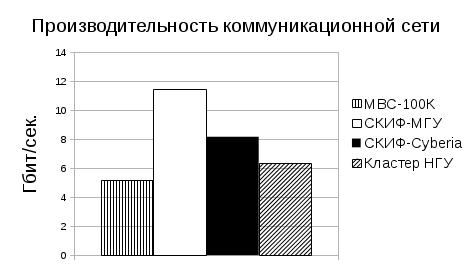
\includegraphics[height=10cm,keepaspectratio]{images/PIC_RAM_Gb_sec.png}
	\end{center}
	\caption{Производительность коммуникационной сети, измеренная на основе скорости пересылки модельных частиц. Измерения выполнены в 2010 г.}
	\label{plot_net_gb_sec}
\end{figure} 

Измеренные данные необходимо сравнивать с заявленными показателями производительности оборудования. Так, производительность сети Infiniband 4x составляла до 32.96 Гбит/с на 2010 г.,  а для Gigabit Ethernet - 10 Гбит/с  

\begin{table}[ht]
	\caption{Сравнение производительности коммуникационной сети, измеренной с помощью теста на основе метода частиц (используются операции MPI\_Send/MPI\_Recv) с характеристиками оборудования.}
	\label{tab_net_gb_sec}
	\begin{tabular}{|c|c|c|c|c|}
		\hline
		             &                     &        &    \multicolumn{2}{|c|}{Производительность,} \\ 
		             &                     & Время            &    \multicolumn{2}{|c|}{Гбит/с} \\ \cline{4-5}              
		Название ВС  & Сеть                & пересылки   & Данные теста       & Максимум  \\
		             &                     & частиц, сек.&   PIC-MANAS        &           \\  \hline
		МВС-100К     &  Infiniband 4x DDR/ &  0.011           &     5.2           & 32       \\ 
		             &  2xGigabit Ethernet/&             &                    &          \\
		             &                     &             &                    &          \\ \hline  
		СКИФ-МГУ     & InfiniBand/         &  0.005           &     11.44          & 32       \\   
		             &  Gigabit Ethernet/  &              &                    &          \\
		             &  СКИФ-ServNet       &              &                    &          \\   
		             &   + IPMI            &             &                     &          \\ \hline  
		СКИФ-Cyberia &  QLogic InfiniPath/ &  0.007           &      8.17              & 10    \\ 
		             &  Gigabit Ethernet/  &             &                    &          \\
		             &  СКИФ-ServNet       &             &                    &          \\ \hline
		Кластер НГУ  & Infiniband 4x DDR/  &  0.009        &     6.35           & 32       \\ 
		             &   Gigabit Ethernet/ &           &                    &          \\
		             &   Gigabit Ethernet  &           &                    &          \\ \hline
	\end{tabular}	
\end{table}

\clearpage

Тем не менее, поскольку не во всех случаях используется эйлерова декомпозиция (геометрическое разделение на подобласти), и соотвественно, измеряется время пересылки модельных частиц, наоборот, во многих случаях достаточно будет ограничится лагранжевой декомпозицией. Таким образом, необходимо иметь также вариант расчета роизводительности коммуникационной сети на основе коллективных операций (MPI\_Allreduce).

В случае лагранжевой декомпозиции выполняется сложение трехмерных массивов тока, вычисленнных каждым процессом по тем модельным частицам, которые принадлежат этому процессу. Таким образом производительность коммуникационной сети при выполнении коллективных операций можно вычислять следующим образом:
\begin{equation}
W_A = \frac{N_X\times N_Y/P_{SUB} \times N_Z \times 24}{T_A}
\label{Net_performance_collective}
\end{equation}

здесь:
\begin{itemize}
	\item $N_X, N_Y, N_Z$ - количество узлов сетки по X,Y и Z соответственно;
	\item $P_{SUB}$ - количество подобластей (если используется эйлерова декомпозиция)
	\item $T_{A}$ - длительность операции MPI\_Allreduce (суммирование токов по всей области), сек.
	\item множитель 24 появляется в силу того, что каждый элемент массива при двойной точности имееет размер 8, и таких массивов 3 (по одному для каждой из компонент тока).
\end{itemize}	

При использовании этой формулы для первого из расчетов, перечисленных в таблице \ref{modern_PIC_params}, можно получить 
$W_A = 1.117$ GB/sec, что закономерно меньше, чем число, полученное для этой же ВС (кластер НГУ) на основе парных пересылок
(таблица \ref{tab_net_gb_sec}).





%		На  рисунке приведено скорость обмена данными между процессами (график из статьи в Мб/сек) 
%		\textbf{перерисовать графики МВС-100К и Ломоносов в общей части}	
%		
%		
%		Сравнение графиков ускорения, полученных на МВС-100К, Ломоносов НГУ и пр.

\section{Оценка возможности выполнения крупномасштабных трехмерных расчетов}
\ref{Big3D}

Проведены тестовые расчеты с целью эффективности распараллеливания и масштабируемости разработанных алгоритмов для моделирования взаимодействия электронного пучка с плазмой, а также с целью выяснения реальных возможностей суперЭВМ по проведению физических расчетов. Показано, что текущая версия программы позволяет проводить расчет на трехмерной сетке размером 350$^3$ узлов при 100 частицах в ячейке за 1 сутки на 10 ядрах суперкомпьютера «Ломоносов», или 42 млн.узлов. Эффективность распараллеливания составила 92 \% для максимального использованного числа ядер: 100 для кластера НГУ и 200 для кластера «Политехник».  















Целью расчетов,  является ответ на вопрос, какие расчеты (т.е. какой размерности) могут бытть проведены на доступных высокопроизводительных  ВС (ВВС), на каком количестве процессоров (или процессорных ядер) и за какое время. 
Для того, чтобы получить ответ на этот вопрос, было запущено большое количество тестовых расчетов. Эти тестовые расчеты носят предварительный характер, и проводятся также с целью выяснения реальных возможностей ВВС для проведения физически содержательных расчетов. 	Расчеты проводились на следующих суперЭВМ: кластер СпбПУ “Политехник”, кластер НКС-1П (ССКЦ СО РАН), кластер НГУ,  суперкомпьютер НИВЦ МГУ “Ломоносов”. 

Основные параметры использованных ВС перечислены в таблице \ref{top50_2018}. Для тех ВС в составе которых имеются различные типы процессоров, указаны те, которые реально использовались в расчетах. Также указана полная пиковая производительность ВС с учетом тех узлов, которые не использовались в данном случае.

\begin{table}[ht]
	\caption{
		Основные характеристики ВС, на которых производились расчеты,рассмотренные в разделах \ref{Big3D} и \ref{complex}, Номера даны по списку Top50 от 03.04.2018 года, В колонке TFLOPS указана пиковая производительность в терафлопсах.}
	\begin{center}
		\begin{tabular}{|c|c|c|c|c|}
			\hline
			
			№ & Название       & Процессор                & Сеть                &  TFlOPS\\
			\hline 
			3 & <<Ломоносов>>  &  2xIntel Xeon 5570       &  Infiniband QDR/   &   1,700.21 \\
			&                &                          &  Gigabit Ethernet/ &            \\
			&                &                          &  Gigabit Ethernet  &            \\ \hline
			
			5 & <<Политехник>> & 2xIntel Xeon CPU E5-2697 &  Infiniband FDR/   &   1,015.10 \\
			&                & 3 GHz                    &  Gigabit Ethernet/ &            \\
			&                & 8.192 GB RAM             &  Gigabit Ethernet  &            \\ \hline
			
			38& НКС-1П         & 2xIntel Xeon E5-2697Av4  & OmniPath           & 91.24      \\
			&                 &                          & Gigabit Ethernet/  &            \\
			&                 &                          & Fast Ethernet      &            \\ \hline
			
			- & Кластер НГУ    & 2xIntel Xeon 5355,       &  Infiniband 4x DDR/& 5.4 \\ 
			&			       &                          &   Gigabit Ethernet/&  \\
			&			       &                          &   Gigabit Ethernet &  \\ \hline                    
			
		\end{tabular}
	\end{center}
	\label{top50_2018}
\end{table}


В ходе проведения тестовых расчетов было получено большое количество числовых характеристик – время расчета для различных сеток (таблица \ref{modern_PIC_params} ), продолжительность коммуникационных операций (рис. 2, 3), эффективность в сильном и слабом смысле (рис.3, 4), причем все это как для лагранжевой, так и для эйлеровой и декомпозиции и для четырех различных суперЭВМ. 






Однако с точки зрения проекта (с точки зрения проведения реальных физических расчетов) имеет смысл только один параметр – оценка размерности расчета продолжительностью 10 тыс. временных шагов,  который можно провести за сутки в данной параллельной конфигурации (при заданном числе процессорных ядер и заданном числе подобластей, на которые разделяется расчетная область), т.е. без увеличения времени коммуникаций. Под размерностью расчета понимается количество узлов N трехмерной кубической сетки (полный размер сетки N*N*N узлов) (одинаковое количество узлов по каждому направлению?) вдоль одного измерения, рис.1. Число частиц во всех тестовых расчетах 100 в ячейке, соответственно и при проведении оценок будем исходить из этого. Размерность расчета оценивается следующим образом:
за основу берется продолжительность временного шага, реально измеренная в ходе тестового расчета
вычисляется отношение времени 8.64 сек. (один шаг из 10 тыс., проводимых за сутки) к измеренной продолжительности временного шага, обозначим это отношение k
размер сетки, реально имеющийся в данном тестовом расчете, умножается на k, и из произведения извлекается кубический корень
в том случае, когда сетка вычисленного размера (вместе с частицами) не помещается в память узла, указывается максимально возможный по объему памяти размер (в основном это касается “Ломоносова”)
Вычисленная таким образом размерность задачи приведена в таблице 1 в выделенной колонке. Кроме того, приведены основные параметры и числовые характеристики тестовых расчетов, обозначенные следующим образом:
\begin{itemize}
	\item $N_X, N_Y, N_Z$  - размер сетки по каждому из измерений
	\item $P_{ALL}$  - общее количество процессорных ядер
	\item $P_{SUB}$  - число подобластей
	\item $T$ – длительность тестового расчета (50 временных шагов), сек.
	\item $\Delta t$  - длительность временного шага, сек.
	\item $T_{A}$ - длительность операции MPI\_Allreduce (суммирование токов по всей области), сек.
	\item $T_{S,B}$ - длительность операции MPI\_Sendrecv (обмен граничными значениями), сек.
	\item $T_{S,PIC}$ - длительность операции MPI\_Sendrecv (пересылка модельных частиц), сек.
\end{itemize}



\begin{table}[ht]
	\begin{center}
		\caption{Время вычислений и время комуникаций в зависимости от числа  процессов.}
		\begin{tabular}{|c|c|c|c|c|c|c|c|c|c|c|c|}
			\hline			
			Кластер & $N_X$ & $N_Y$ & $N_Z$ &$P_{ALL}$  & $P_{SUB}$ & $T$ & $\Delta t$ & $T_{A}$ &  $T_{S,B}$ & $T_{S,PIC}$ \\\hline
			НГУ     & 100   & 100   & 20    &  1        & 1         & 39.1  & 0.78 & 0.004         & 0      &    \\\hline
			НГУ     & 100   & 100   & 20    &  2        & 1         & 21.49 & 0.42 & 0.0029         & 0     &    \\\hline
			НГУ     & 100   & 100   & 20    &  2        & 2         & 40.37 & 0.8 & 0.097         & 0.022   &    \\\hline
			НГУ     & 100   & 100   & 20    &  4        & 1         & 9.9 & 0.19 & 0.0036         & 0       &    \\\hline
			НГУ     & 100   & 100   & 20    &  4        & 2         & 16.1 & 0.32 & 0.004         & 0.0094  &    \\\hline
			НГУ     & 100   & 100   & 20    &  10       & 1         & 6.7 & 0.13 & 0.0026         & 0       &    \\\hline
			НГУ     & 100   & 100   & 20    &  100      & 1         & 4.0   & 0.08 & 0.0059         & 0     &    \\\hline
			НГУ     & 500   & 500   & 20    &  20       & 1         & 714.9 & 14.2 & 6.89         & 0       &    \\\hline
			<<Политехник>> & 100   & 100   & 20    &  4       & 2         & 13.8 & 0.27 & 0.0069  & 0.0035  &    \\\hline
			<<Политехник>> & 100   & 100   & 20    &  100     & 10        & 2.4 & 0.048 & 0.00223 & 0.001   &    \\\hline
			<<Политехник>> & 500   & 500   & 20    &  50       & 5        & 70.7 & 1.4 & 0.0014   & 0.006   &    \\\hline
			<<Политехник>> & 500   & 500   & 20    &  100       & 10      & 64.0 & 1.28 & 0.054   & 0.029   &    \\\hline
			<<Политехник>> & 500   & 500   & 20    &  200       & 20      & 70.2 & 1.4 & 0.096    & 0.009   &    \\\hline
			<<Ломоносов>> & 100   & 100   & 20    &  10       & 1         & 2.0 & 0.04 & 0.003    & 0       &    \\\hline
			<<Ломоносов>> & 100   & 100   & 20    &  100       & 1        & 2.5 & 0.05 & 0.005    & 0       &    \\\hline
			НКС-1П        & 100   & 100   & 20    &  100       & 1        & 28.9 & 0.57 & 0.0075  & 0       &    \\\hline
			НКС-1П        & 100   & 100   & 20    &  200       & 1        & 35.1 & 0.7 & 0.069    & 0       &    \\\hline
			
		\end{tabular}
	\end{center}
	\label{modern_PIC_params}
\end{table}

\begin{figure}[htb]
	\begin{center}
		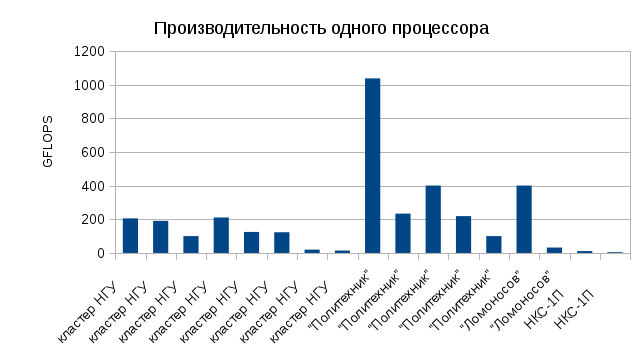
\includegraphics[height=10cm,keepaspectratio]{images/modern_PIC_params_FLOPS.png}
	\end{center}
	\caption{Критерий комплексной оценки пригодности ВС для решения задач математического моделирования.}
	\label{xi}
\end{figure} 

\clearpage

\textbf{ прогноз эффективности на лин. ур, сравнениес топ50 - должны совпасть б/м}






\section{Формула для комплексной оценки ВС}
\label{complex_evaluation}
В \textit{четвертом разделе} приведено обоснование формулы, на основании которой выносится оценка ВС по материалам проведенных тестов. При этом важно отметить, что оценка является не сравнительной - относительно других ВС, а абсолютной - с точки зрения математического моделирования. 

В частности, для того, чтобы параллельная ВС могла быть признана адаптированной к задачам математического моделирования, она должна соответвовать следующим требованиям:
\begin{enumerate}
	\item Очень высокая производительность коммуникационной сети ($W_S$, формула \ref{Net_performance_peer} и $W_A$, формула \ref{Net_performance_сollective} ), позволяющая пересылать все необходимые для расчета данные, не задерживая вычислений;
	
	\item Относительно высокая производительность оперативной памяти ($W_{PIC,GB/sec}$, формула \ref{RAM_performance}), позволяющая эффективно использовать ресурсы процессоров, т.е. фактически совпадающая с производительностью процессора.  	
\end{enumerate}

Важно отметить, что названы относительные показатели, обеспечивающие возможность пересылать данные, без ущерба для скорости вычислений. Именно это и означает  комплексную пригодность ВС к решению задач математического моделирования.

В случае использования эйлеро-лагранжевой декомпозиции, т.е. если определены обе величины $W_S$ и $W_A$, будем использовать усредненную величину
\begin{equation}
W_{MPI} = \frac{W_S + W_A}{2}
\end{equation}
в случае только лишь эйлеровой или только лагранжевой декомпозиции, $W_{MPI}$ равна соотвественно, $W_S$ или $W_A$

В итоге предлагается формула оценки $\xi$ в виде:
$$
\xi = \frac{W_{MPI}} { W_{PIC,GB/sec}}, 
$$
Комплекснная оценка ВС, вычисленная по формуле \ref{complex_rating}
на материале расчетов, показанных в таблице \ref{modern_PIC_params}
показана на рисунке \ref{xi}

\begin{figure}[htb]
	\begin{center}
		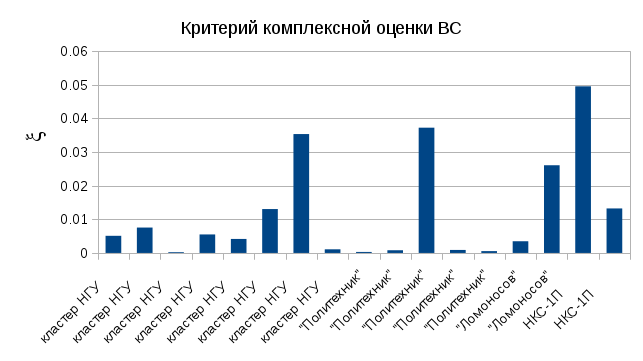
\includegraphics[height=10cm,keepaspectratio]{images/modern_PIC_params_xi.png}
	\end{center}
	\caption{Критерий комплексной оценки пригодности ВС для решения задач математического моделирования.}
	\label{xi}
\end{figure} 
Данный критерий, напомним, выражает степень сбалансированности производительности процессоров ВС и коммуникационной системы. Поэтому он может быть низким для некоторых ВС, стоящих высоко в рейтинге Top50.

Вместе тем особую важность представляет вопрос о соответствии нового критерия известным и часто используемым характеристикам ВС, таким как вычислительная производительность (в единицах GFLOPS) и параллельная эффективность. Взаимосвязь этих величин и критерия комплексной оценки интуитивно ясна, но\textbf{ требуется выявить ее количественно????}

посчитать его для хорошего графика эффективности на Ломоносов-GPUи для плохого на МВС-100К. ДОЛжна быть сущесвенная разница.

так же и по флопсам на основе FDTD.


\section{Сравнение с известными тестами производительности}

\subsection{Тест HPL}

\subsubsection{Краткое описание теста HPL}
Тест HPL (High Performance Linpack) - это многопроцессорный вариант широко известного теста Linpack. В свою очередь Linpack - это набор вычислений с использованием матричного умножения, который масштабирует размер массивов, чтобы попытаться создать максимально возможную нагрузку для вычислительной системы и таким образом достичь максимальной производительности на всех процессорных элементах в кластере. Вначале в рамках теста Linpack решалась система линейных уравнений с плотной матрицей размером $ 100 \times 100$, затем по мере роста производительности разиерность была увеличена до $ 100 \times 100$ она переходила к 1000 x 1000, когда машины становились более мощными.

\subsubsection{Результаты тестирования кластера НГУ на тесте HPL}
\subsubsection{Результаты тестирования кластера СПбПУ <<Политехник>> на тесте HPL}
\subsubsection{Результаты тестирования кластера НКС-1П на тесте IMB}
\subsection{Тест HPCG}
Тест HPCG представляет собой предобусловленный метод сопряженных градиентов
(англ., Preconditioned Conjugate Gradient, PCG) с локальным симметричным предобуславливателем Гаусса-Зейделя, реализованный на C ++ 2 с использованием MPI и OpenMP. 

HPCG (High Performance Conjugate Gradient) \cite{Dongarra2016HighperformanceCB} - это сравнительно новый тест производительности высокопроизводительных вычислительных систем (ВВС), претедующий на более адекватное по сравнению с наиболее часто используемым тестом HPL.

Определенные соображения по поводу того, почему HPCG может заменить HPL при составлении рейтинга высокопроизводительных вычислительных систем, были высказаны в статье \cite{HPCGreplaceHPL}. Они заключаются в следующем. Тесты, выполняемые на ВВС должны позаолять произвести сравнительное ранжирование систем с точки зрения производительности по различным архитектурам и пакетам программного обеспечения, и давать некоторое представление о производительности относительно финансовых и временных затрат для разных систем, чтобы пользователи могли взвешивать относительную экономическую целесообразность вычислительных систем, которые могут запускать конкретное приложение. К сожалению, выполняемы на высокопроизводительных ВС тесты, в основном делают первое, и редко делают второе. 

Автор теста HPCG Джек Донгарра говорит \cite{Dongarra2016HighperformanceCB}, что проблемы с текущими рейтингами на основе LinPack (или , что то же самое HPL) в том, что они уже не так сильно коррелируют с реальной производительностью приложений, особенно для широкого набора приложений HPC, на основе решения дифференциальных уравнений, которые нуждаются в гораздо более высокой пропускной способности и низкой латентности, и имеют вс е более нерегулярный доступа к данным. Таким образом, проектирование ВВС на основе HPL может привести к плохой производительности для реальных приложений или добавлению ненужной сложности в систему.


\subsubsection{Актуальность создания нового теста для определения производительности ВВС}
Необходимость создания нового теста (а именно, HPCG) для ранжирования ВВС его авторы формулируют следующим образом, \cite{HerouxHPCG}. В данном случае имеет смысл привести длинную цитату по той причине, что диссертационная работа также посвящена созданию нового теста для ВВС, и для вновь создаваемого теста PIC-MANAS актуальны все те же самые соображения.

Итак, тест HPCG:
<<1.Обеспечивает охват основных коммуникационных и вычислительных моделей:
основные виды коммуникаций (глобальные и локальные коллективные комуникации) и вычислительные модели
(векторные сложения, точечные произведения, умножения разреженных матриц на вектора и локальные решение систем линейных уравнений с треугольными матрицами), присутствующие в наших кодах для решения дифференциальных уравнений с использрванием как явных, так и неявных методов,
присутствуют в этом тесте. Возникающие асинхронные коллективные коммуникации и другие операции со скрытой латентностью методы могут быть изучены в контексте HPCG, и таким образом будет внесен вклад в оптимизацию будущих вычислительных систем.

2. Представляет собой минимальный набор основных вычислительных моделей: HPCG является наименьшим
эталонным кодом, содержащим эти основные шаблоны, и в то же время представляющий собой
реальные математические вычисления.

3. Показывает результаты повышения эффективности коллективных опреаций, зависящих от пропускной способности внутренней сети ВС. Определение соседства и редукция представляют собой существенные затруднения для многих приложений. Таким образом, повышение производительности на тесте HPCG будет
имеет серезную корреляцию с улучшить производительность наших реальных приложений.

4. Показывает результаты повышения эффективности локальной памяти: производительность процессора
на тесте HPCG во многом определяется эффективным использованием локальной памяти.
Усовершенствования в реализации структур данных HPCG, компиляция кода HPCG
кода и производительности системы в целом улучшит базовый уровень результатов HPCG
в вместе с этим производительность реальных приложений, а также проинформирует разработчиков приложений о новых подходах к оптимизации.
5. Обнаруживает и измеряет отклонения от побитовых совпадения резульатов вычислений.
СУществует опасение, что будущие компьютерные системы не смогут обеспечить детерминированное исполнение
 вычислений с плавающей точкой. Поскольку сложение с плавающей точкой не является ассоциативным,
это означает, что мы, как правило, не будем иметь побитовые воспроизводимые результаты, даже при повторном исполнении на том же числе процессоров одной и той же системы.
Это важное отличие от многих приложений MPI сегодня, и представляет большой
вызов приложениям, которые должны сертифицировать свои вычислительные результаты. В тесте  HPCG нарушение побитовой воспроизводимости очевидно. >>

Легко заметить что высказанные авторами теста HPCG соображения во многом похожи на содержание раздела <<Актуальность>> во введении настоящей работы. Важное отличие теста PIC-MANAS от HPCG заключается в том, что позволяет четко определяеть, какая именно из подсистем ВС (память, коммуникационная подсистема, процессоры) оказывает основное влияние на снижение производительности, а не просто в целом реагирует на оптимизацию их работы, как описано выше в пунктах 3 и 4.

 
\subsubsection{Результаты тестирования кластера СПбПУ <<Политехник>> на тесте HPCG}